A ``cold box'' at CERN used in electronics tests for ProtoDUNE-SP is available for electronics testing in cold nitrogen gas. The cold box is designed to cycle one full-size DUNE APA with the full compliment of 20 FEMB through gaseous nitrogen temperatures around 150K to check out the APA performance prior to installing the APA into the ProtoDUNE-SP cryostat. It is designed to be a Faraday cage identical to the ProtoDUNE-SP cryostat and is read out by a complete CE system for a single APA, including a CE flange and fully-loaded WIEC with 5 WIBs and 1 PTC.

Preliminary results from the ProtoDUNE-SP cold box indicate that
the noise performance of the TPC readout will satisfy the DUNE FD noise requirements of
ENC~<~1000e$^-$ on DUNE length wires. These measurements suggest that the noise level in
LAr would be around 500e$^-$ and 600e$^-$ for the collection and induction plane channels,
respectively; this is well below the requirement.  The ENC and temperature of the second ProtoDUNE-SP
APA delivered to CERN in the cold box are shown in Figure~\ref{fig:cb_results}.

\begin{dunefigure}
[ENC in electrons (left axis) for the wrapped induction wires (red and blue curves) and 
straight collection wires (green) and temperature in degrees Kelvin (right axis) for the temperature
sensors in the CERN cold box (orange curves) as a function of cold cycle time in GN2 for ProtoDUNE-SP APA2. 
At the lowest temperature of 160K, the wrapped wires measured 480e$^-$ noise and the straight 
wires 400e$^-$. This noise level is consistent with all other ProtoDUNE-SP APAs tested in the cold box.]
{fig:cb_results}
{ENC in electrons (left axis) for the wrapped induction wires (red and blue curves) and 
straight collection wires (green) and temperature in degrees Kelvin (right axis) for the temperature
sensors in the CERN cold box (orange curves) as a function of cold cycle time in GN2 for ProtoDUNE-SP APA2. 
At the lowest temperature of 160K, the wrapped wires measured 480e$^-$ noise and the straight 
wires 400e$^-$. This noise level is consistent with all other ProtoDUNE-SP APAs tested in the cold box.}
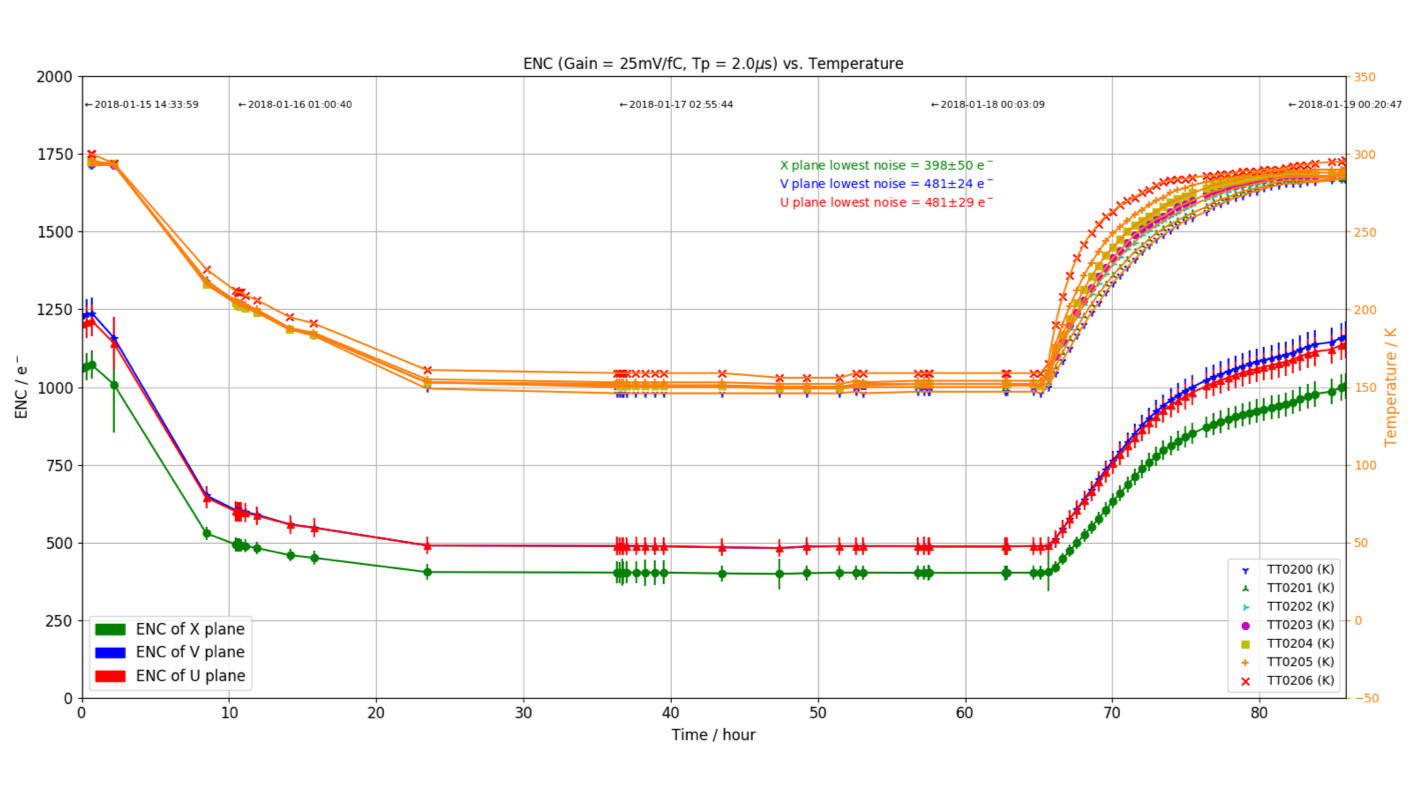
\includegraphics[width=0.9\linewidth]{tpcelec-apa2-results.png}
\end{dunefigure}
